\documentclass[12pt]{article}

\usepackage{amsmath}
\usepackage{graphicx}
\usepackage{caption}
\usepackage{subcaption}
\usepackage{enumerate}
\usepackage{rotating}
\usepackage{multirow}
\usepackage{booktabs}
\usepackage{parskip}
\usepackage{endnotes}
\usepackage{setspace}
\usepackage{dcolumn} %for use with R package stargazer
\interfootnotelinepenalty=10000
\usepackage[top=1in,bottom=1in,left=1in,right=1in]{geometry}

\newcommand{\yoverbrace}[2][\vphantom{\beta_{1pi}T + \mu_{pit}}]{\overbrace{#1#2}}

\newcommand{\lefttext}[1]{\makebox[0pt][l]{#1}}

\usepackage{natbib}
\usepackage{hyperref}
\hypersetup{pdfstartpage=1,
            pdfpagemode=UseNone,
            pdfstartview=FitH,
            pdffitwindow=true,
            urlcolor=blue,
            bookmarks=false,
            urlcolor=blue,
            colorlinks=true,
            linkcolor=blue,
            citecolor=blue}

\usepackage{lastpage}
\usepackage{fancyhdr}
\usepackage{afterpage}
\pagestyle{fancy}
\fancyhead{} % clear all header fields
\fancyfoot{} % clear all footer fields
\fancyhead[L]{Latner}
\fancyhead[C]{Economic insecurity}
\fancyhead[R]{Page \thepage\  of \pageref*{LastPage}}
\renewcommand{\headrulewidth}{0pt}
\renewcommand{\footrulewidth}{0pt}

\fancypagestyle{firststyle}
{
   \fancyhead{}
   \fancyfoot{}
}


\begin{document}

\afterpage{\cfoot{\thepage}}

{\bf  Revision date:} \today

\begin{center}
\large Economic insecurity and the distribution of income volatility in the United States \\
\bigskip
\normalsize
Jonathan P. Latner $^{a}$\\
\end{center}

%%%%%%%%%%%%%%%%%%%%%%%%%%
% SECTION
%%%%%%%%%%%%%%%%%%%%%%%%%%
{\bf  Abstract}

We examine inequalities in the distribution of income volatility in two ways using data from the Panel Study of Income Dynamics (PSID) in order to improve our understanding of economic insecurity.  First, we use a variance function regression to jointly quantify the relationship between changes in average levels of volatility as they relate to changes in the distribution of volatility. The results indicate that inequalities in the distribution of volatility rise much faster than the overall level of volatility.  Therefore, the concern is less about rising income volatility and more about the characteristics of who experiences high levels of volatility and how those characteristics are changing over time.  Second, we use a linear probability model to better understand changes in who experiences high income volatility over time.  Rising inequalities in the distribution of volatility turn out to be the result of a rising probability of experiencing high volatility among households that would not typically be classified as economically insecure.  

{\bf  Keywords:} income volatility, income mobility, inequality, economic insecurity, standard of living

Please cite as: Latner, Jonathan (2019).  ``Economic insecurity and the distribution of income volatility in the United States.'' \emph{Social Science Research}, 77:193-213

\vfill

------------------------ \\
\footnotesize
$^{a}$ Corresponding author: Jonathan P. Latner.  E-mail:  \url{jonathan.latner@uni-bamberg.de}\\
The author wishes to acknowledge the following individuals for their help throughout the entire process (in alphabetical order):  Hilke Brockmann, David Calnitsky, Matias Cocina, Martin Ehlert, Sophia Fauser, Markus Gangl, Ted Gerber, Pilar Gonalons-Pons, Michael Gebel, Eric Grodsky, Andreas Haupt, Richard Latner, Fabian Ochsenfeld, Ellen Pechman, Sonja Scheuring, Jody Schimek, Xi Song, Tim Smeeding, Leann Tigges, Jonas Vo{\ss}emer, Trevor Young-Hyman, and the anonymous reviewers.

\clearpage
%%%%%%%%%%%%%%%%%%%%%%%%%%%%%%%%
% TABLES
%%%%%%%%%%%%%%%%%%%%%%%%%%%%%%%%
\section{Tables}

\begin{table}[!ht]
    \caption{Descriptive statistics}
    \begin{center}
    \resizebox{\textwidth}{!}{
\begin{tabular}{@{\extracolsep{0pt}}lD{.}{.}{-3} D{.}{.}{-3} D{.}{.}{-3} D{.}{.}{-3} D{.}{.}{-3} D{.}{.}{-3} } 
\\[-1.8ex]\hline 
\hline \\[-1.8ex] 
Statistic & \multicolumn{1}{c}{N} & \multicolumn{1}{c}{Mean} & \multicolumn{1}{c}{St. Dev.} & \multicolumn{1}{c}{Pctl(25)} & \multicolumn{1}{c}{Median} & \multicolumn{1}{c}{Pctl(75)} \\ 
\hline \\[-1.8ex] 
\multicolumn{7}{l}{\emph{Income characteristics (household):}} \\ 
                \hspace{10mm} $^{1}$Income at start ($y_{pi}$) & 48,718 & 21,998.110 & 24,619.800 & 8,605.846 & 15,614.340 & 27,705.030 \\ 
\hspace{10mm} $^{2}$Log income at start ($y_{pi}$) & 48,718 & 0.000 & 64.037 & -36.127 & 3.836 & 41.595 \\ 
\multicolumn{7}{l}{\phantom{empty}} \\ 
              \hspace{10mm} $^{3}$Change in income ($\Delta \hat{y}_{pi}$) & 48,718 & 0.000 & .570 & -.305 & .013 & .328 \\ 
\hspace{10mm} $\Delta \hat{y}_{pi} >$ 5\% & 22,788 & .444 & .359 & .190 & .352 & .591 \\ 
\hspace{10mm} $\Delta \hat{y}_{pi} <$ -5\% & 21,622 & .468 & .412 & .184 & .353 & .616 \\ 
\multicolumn{7}{l}{\phantom{empty}} \\ 
                \hspace{10mm} $^{4}$Income volatility ($\upsilon_{pi}$) & 48,718 & 23.437 & 17.207 & 12.414 & 18.883 & 28.891 \\ 
\hspace{10mm} Income volatility (Log $\upsilon_{pi}$) & 48,718 & 2.944 & .646 & 2.519 & 2.938 & 3.364 \\ 
\hspace{10mm} High income volatility ($\upsilon_{pi} > 90^{th}$ pct) & 48,718 & .100 & .300 & 0 & 0 & 0 \\ 
\multicolumn{7}{l}{\phantom{empty}} \\ 
             \multicolumn{7}{l}{\emph{Demographic characteristics (head):}} \\ 
             \hspace{10mm} Male & 48,718 & .868 & .338 & 1 & 1 & 1 \\ 
\multicolumn{7}{l}{\phantom{empty}} \\ 
             \hspace{10mm} White & 48,718 & .692 & .462 & 0 & 1 & 1 \\ 
\multicolumn{7}{l}{\phantom{empty}} \\ 
                \hspace{10mm} Less than HS & 48,718 & .183 & .386 & 0 & 0 & 0 \\ 
\hspace{10mm} HS & 48,718 & .355 & .478 & 0 & 0 & 1 \\ 
\hspace{10mm} More than HS & 48,718 & .462 & .499 & 0 & 0 & 1 \\ 
\multicolumn{7}{l}{\phantom{empty}} \\ 
              \hspace{10mm} Older (Age $>$49) & 48,718 & .074 & .262 & 0 & 0 & 0 \\ 
\multicolumn{7}{l}{\phantom{empty}} \\ 
                \multicolumn{7}{l}{\emph{Family characteristics (In a study period):}} \\
                \hspace{10mm} Always single & 48,718 & .173 & .378 & 0 & 0 & 0 \\ 
\hspace{10mm} Marital change & 48,718 & .166 & .372 & 0 & 0 & 0 \\ 
\hspace{10mm} Always married & 48,718 & .661 & .473 & 0 & 1 & 1 \\ 
\multicolumn{7}{l}{\phantom{empty}} \\ 
                \hspace{10mm} Never kids & 48,718 & .422 & .494 & 0 & 0 & 1 \\ 
\hspace{10mm} Sometimes kids & 48,718 & .192 & .394 & 0 & 0 & 0 \\ 
\hspace{10mm} Always kids & 48,718 & .386 & .487 & 0 & 0 & 1 \\ 
\multicolumn{7}{l}{\phantom{empty}} \\ 
               \multicolumn{7}{l}{\emph{Employment characteristics (In a study period):}} \\
               \hspace{10mm} Ever unemployed & 48,718 & .387 & .487 & 0 & 0 & 1 \\ 
\multicolumn{7}{l}{\phantom{empty}} \\ 
              \hspace{10mm} Ever self employed & 48,718 & .274 & .446 & 0 & 0 & 1 \\ 
\hline \\[-1.8ex] 
\hspace{3mm}Total N & \multicolumn{1}{l}{48,718} & & & & \\
\hspace{3mm}Unique N & \multicolumn{1}{l}{6,638} & & & & \\
\hspace{3mm}Avg. study periods per unique N & \multicolumn{1}{l}{11.94} & & & & \\
\hline \\[-1.8ex]

\multicolumn{7}{l}{$^1$ The average of the first two-observations in a study period.  Income is family size adjusted.} \\
\multicolumn{7}{l}{$^2$ The residual of log income after taking out year fixed effects in a given study period for the first year of a given study period.} \\
\multicolumn{7}{l}{$^3$ Where $\Delta \hat{y}_{pi} = \hat{y}_{pi,t=N} - \hat{y}_{pi,t=1}$ if $\hat{y}_{pit} = \beta_{0i} + \beta_{1i} T$} \\
\multicolumn{7}{l}{$^4$ Where $\upsilon_{pi} = \text{\emph{Standard deviation }} (\mu_{pit})$ if $\text{log } y_{pit} = \beta_{0pi} + \beta_{1pi} T + \mu_{pit}$}
\end{tabular} 
}
    \label{descriptives}
    \end{center}
\end{table}

\begin{table}[!ht]
    \caption{Determinants of average level of income volatility and the distribution of volatility, parameter estimates from a variance function regression with fixed effects}
    \begin{center}
    \resizebox{\textwidth}{!}{
\begin{tabular}{@{\extracolsep{5pt}}lD{.}{.}{-3} D{.}{.}{-3} } 
\\[-1.8ex]\hline 
\hline \\ [-1.8ex] & \multicolumn{1}{c}{Average ($\beta$)} & \multicolumn{1}{c}{Distribution ($\lambda$)} \\
\hline \\[-1.8ex] 
 Downward mobility ($\Delta \hat{y}_{pi} < -5$) & 0.315$ $(0.007) & -0.188$ $(0.039) \\ 
  & & \\ Upward mobility ($\Delta \hat{y}_{pi} > 5)$ & 0.118$ $(0.008) & -0.102$ $(0.046) \\ 
  & & \\ Income at start & -0.157$ $(0.008) & 0.063$ $(0.045) \\ 
  & & \\ Older (Age $>$ 49) & 0.009$ $(0.009) & 0.413$ $(0.047) \\ 
  & & \\ 
                         \emph{Study period beginning:} & & \\
                         \hspace{10mm} 1975 $-$ 1979 & 0.011$ $(0.006) & -0.263$ $(0.036) \\ 
  \hspace{10mm} 1980 $-$ 1984 & 0.025$ $(0.007) & -0.216$ $(0.041) \\ 
  \hspace{10mm} 1985 $-$ 1989 & 0.091$ $(0.008) & -0.137$ $(0.046) \\ 
  \hspace{10mm} 1990 $-$ 1996 & 0.111$ $(0.009) & 0.232$ $(0.053) \\ 
  \hspace{10mm} 1997 $-$ 2003 & 0.040$ $(0.010) & 0.345$ $(0.059) \\ 
  & & \\ 
                    Constant & -0.000$ $(0.002) & -2.108$ $(0.009) \\ 
 \hline \\[-1.8ex] 
Observations & \multicolumn{1}{c}{48,718} & \multicolumn{1}{c}{48,718} \\ 
R$^{2}$ & \multicolumn{1}{c}{0.057} &  \\ 
\hline 
\hline \\[-1.8ex] 
\textit{Note:}  & \multicolumn{2}{l}{Standard errors in parenthesis.} \\ 
\end{tabular} 
}
    \label{vfr_fe}
    \end{center}
\end{table}

\clearpage
%%%%%%%%%%%%%%%%%%%%%%%%%%%%%%%%
% FIGURES
%%%%%%%%%%%%%%%%%%%%%%%%%%%%%%%%
\section{Figures}

%do stata -b do ../../../../do_files/distribution/graph_inequality.do
\begin{figure}[htp!]
    \centering
    \caption{Index of trends in income volatility and distribution of volatility}
    \resizebox{.9\textwidth}{!}{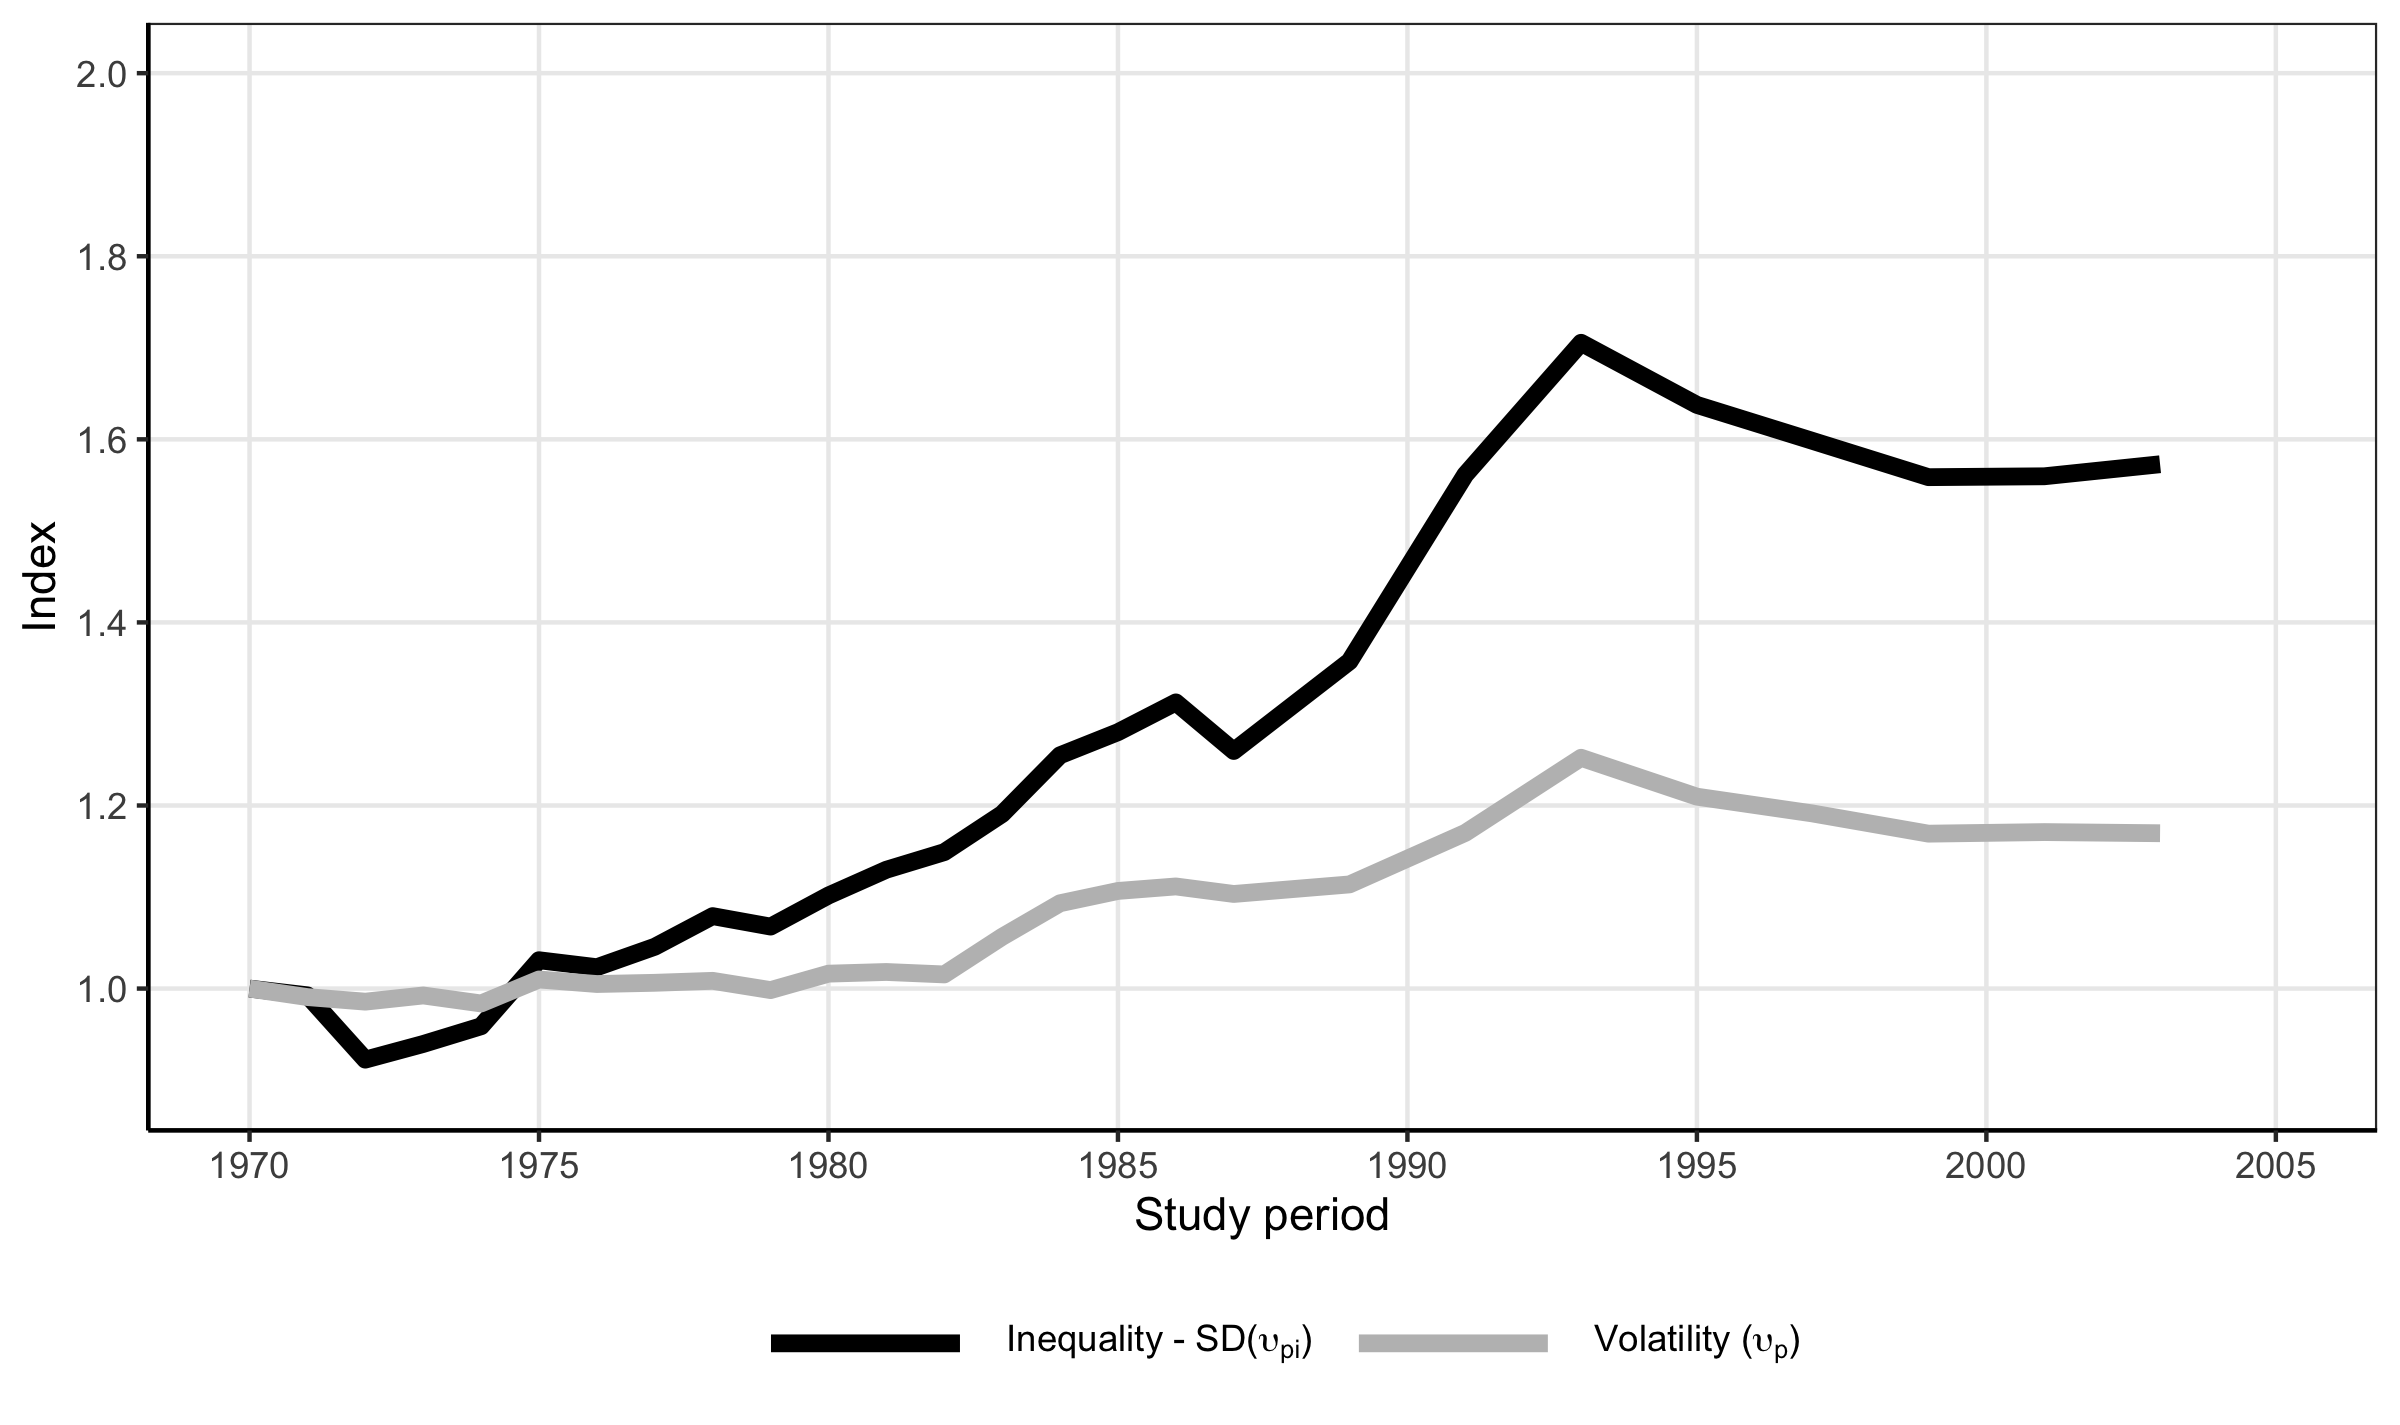
\includegraphics{../graphs/volatility_and_inequality_trends_hh.png}}
    \label{index_volatility}
\end{figure}

\begin{figure}[htp!]
    \captionsetup[subfigure]{position=b}
    \caption{Relationship between the level and distribution of volatility and mobility, as shown in table \ref{vfr_fe}}
    \subcaptionbox{Average volatility}{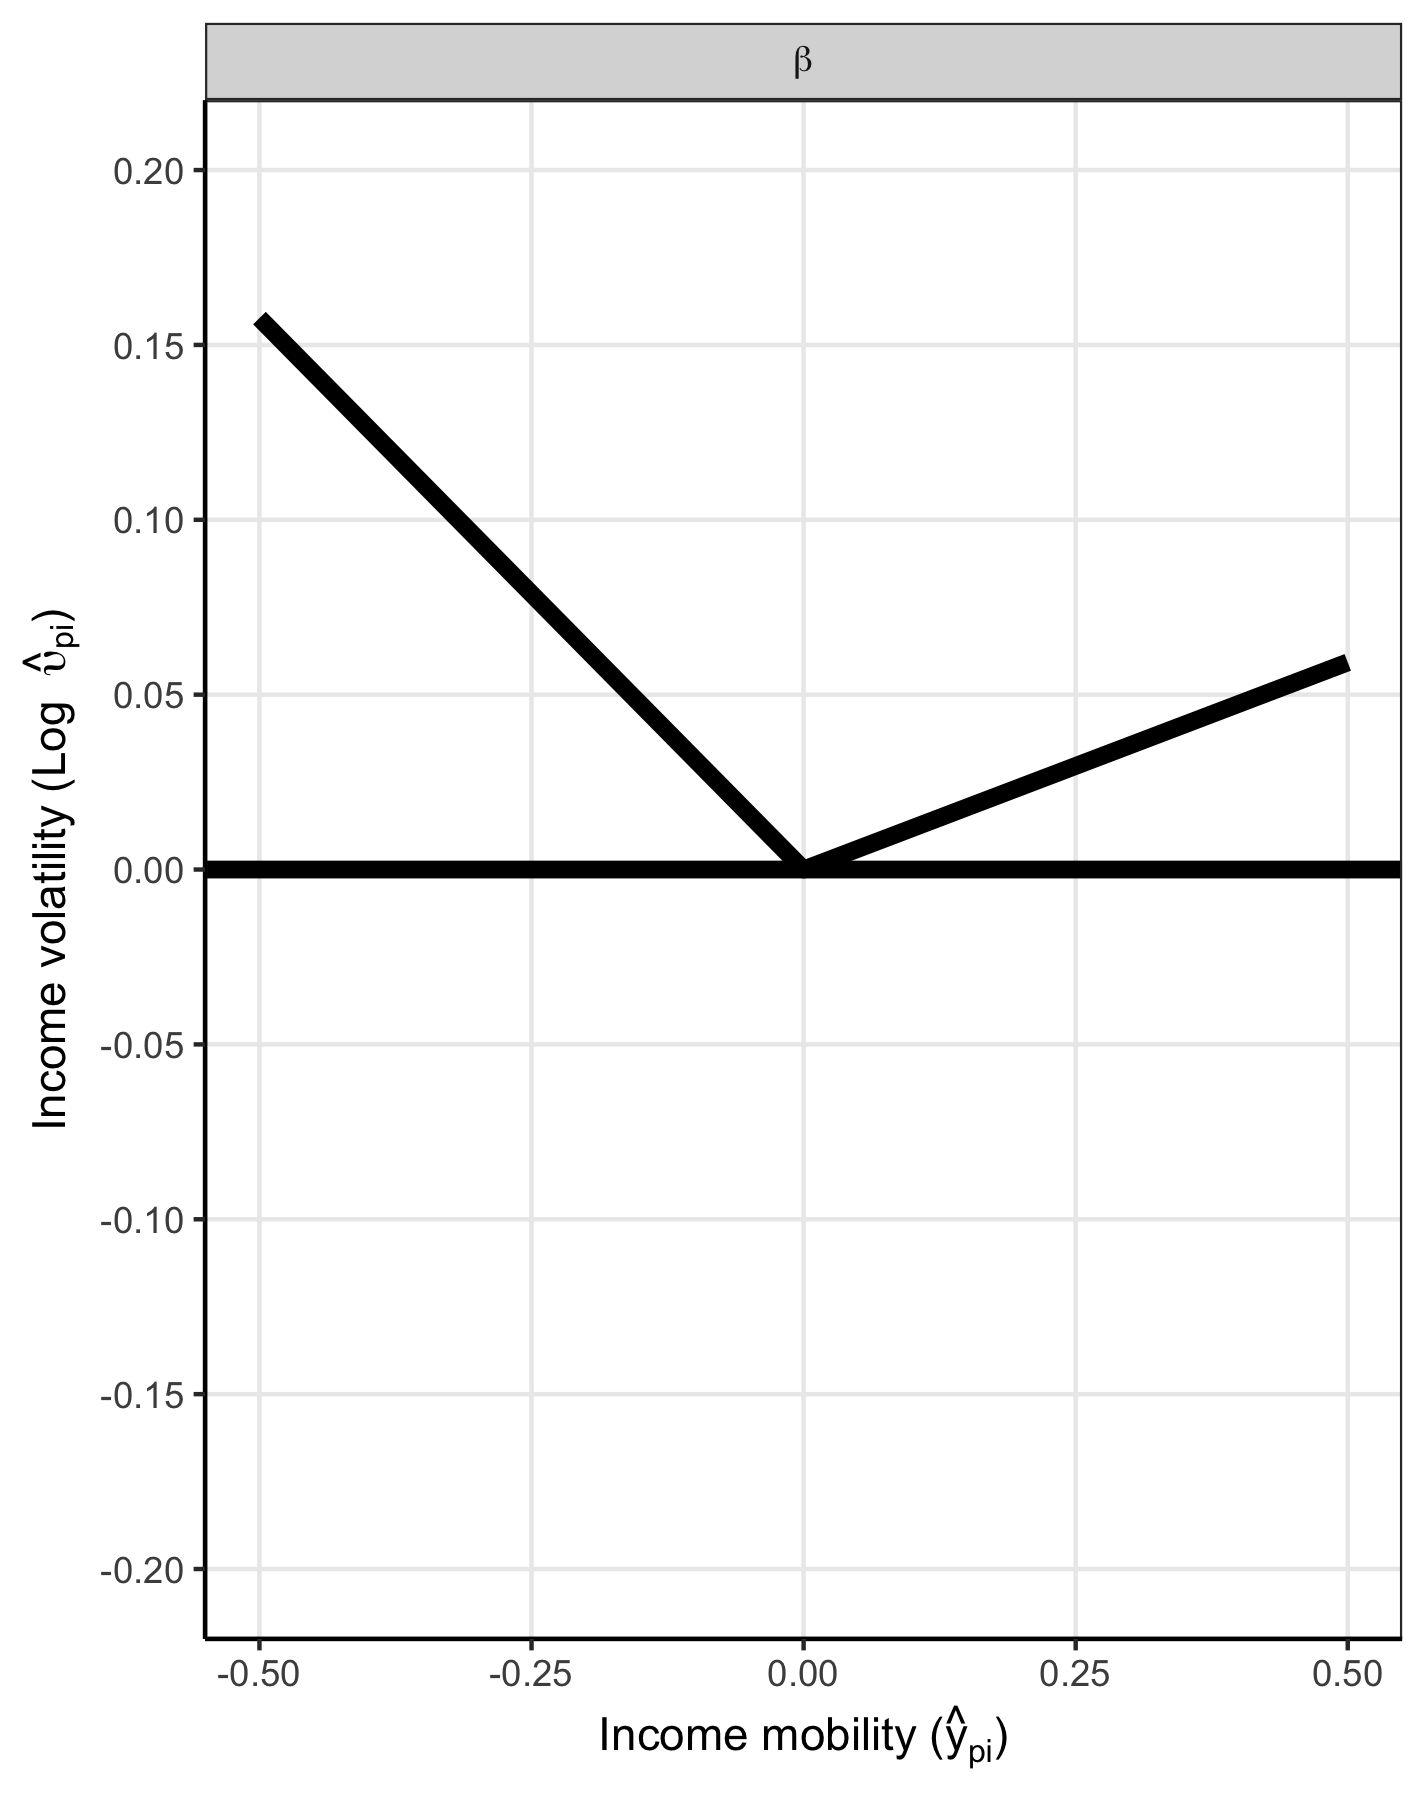
\includegraphics[width=0.475\textwidth]{../graphs/margins_betas_fe.png}}
    \hfill
    \subcaptionbox{Distribution of volatility}{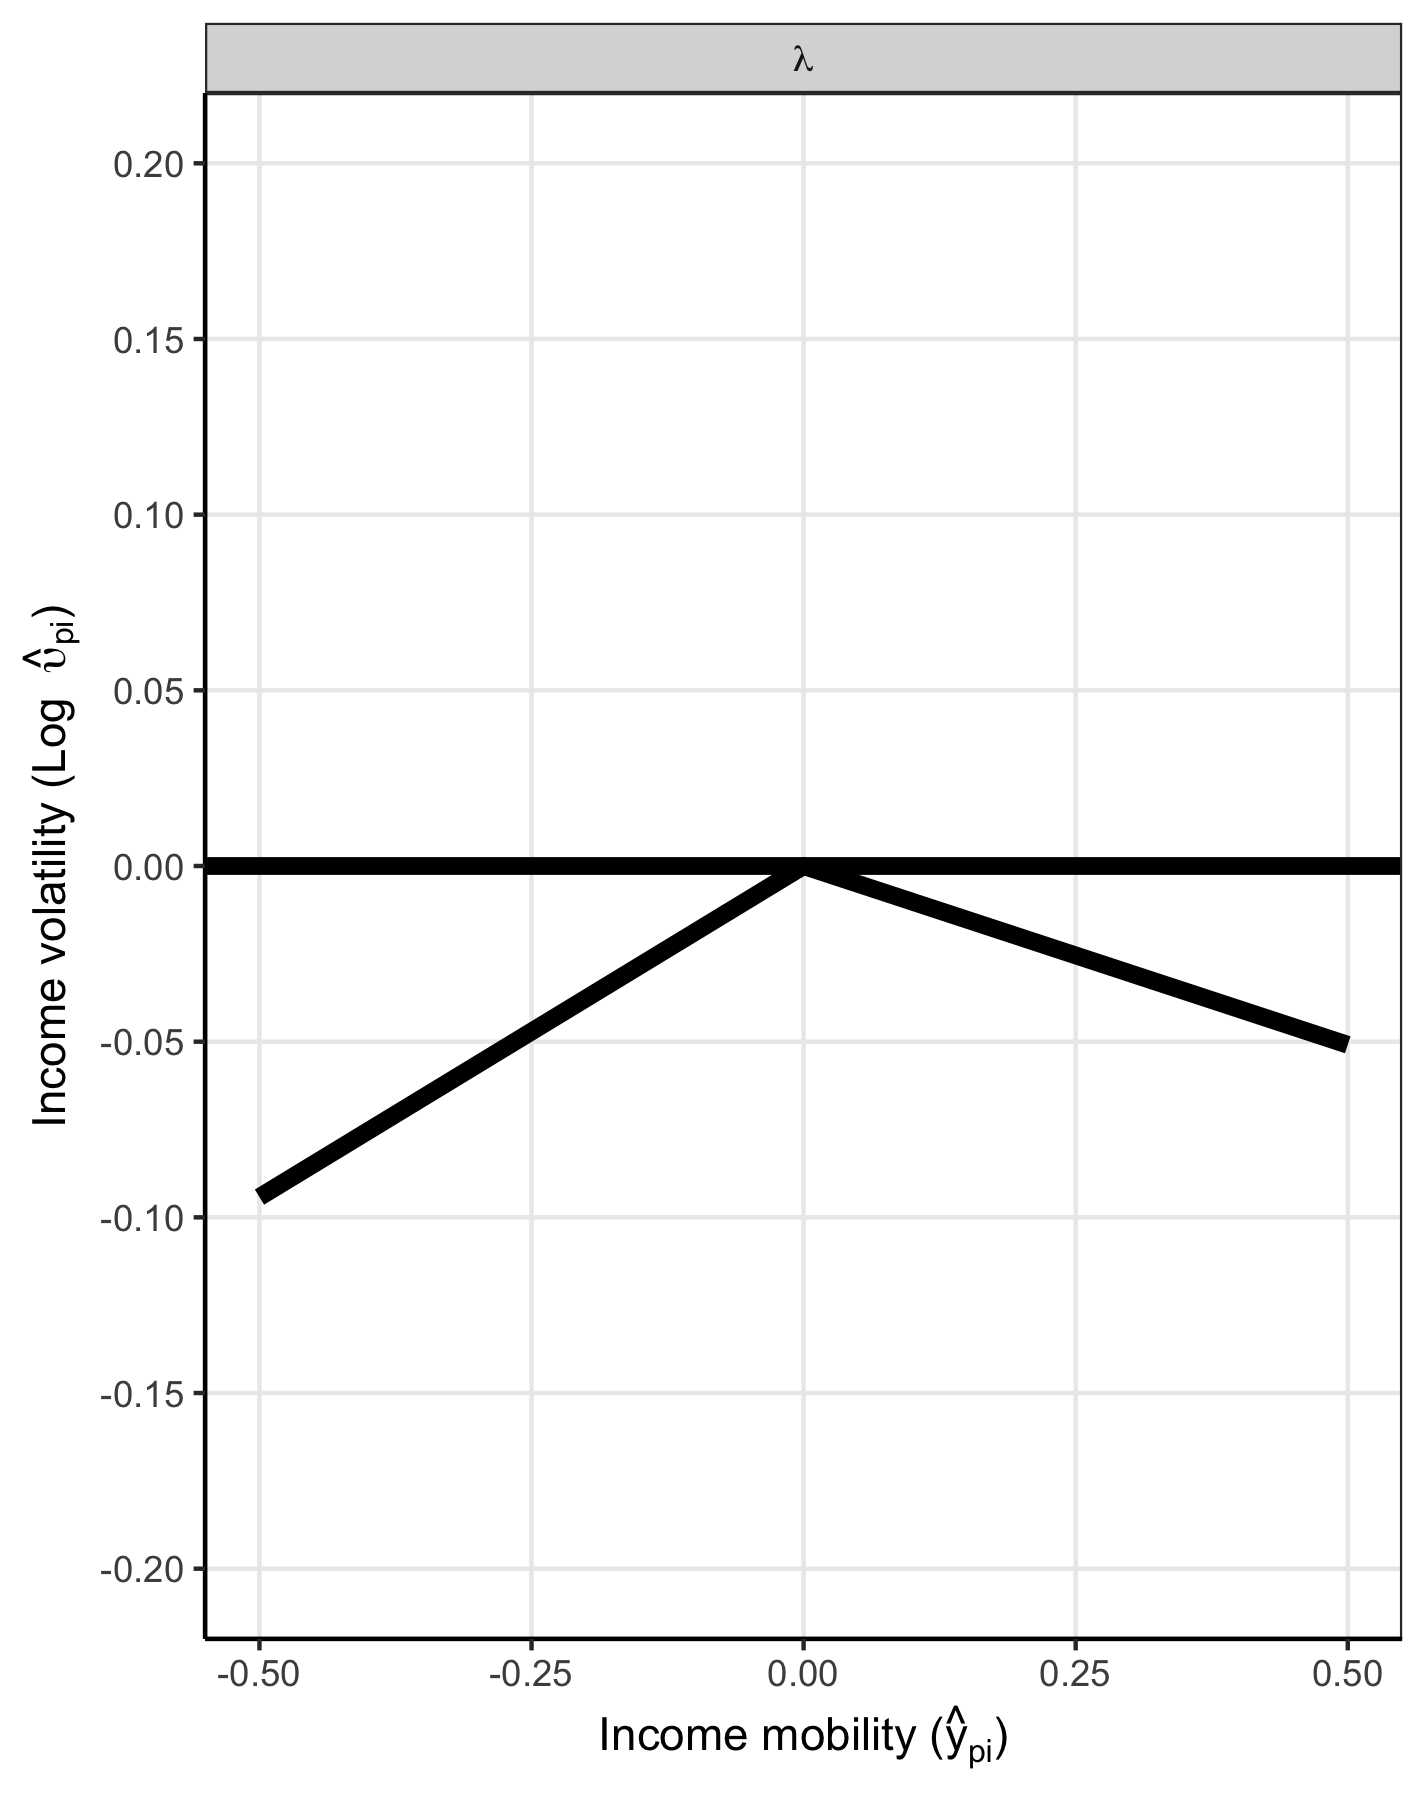
\includegraphics[width=0.475\textwidth]{../graphs/margins_lambdas_fe.png}}
    \label{margins_beta_lambda}
    \\\\
    \raggedright{\footnotesize{Note: Graph illustrates the impact of a percentage change in income mobility on the level and distribution of income volatility from table \ref{vfr_fe}, if all other continuous variables are at their average values and the categorical variables are at their baseline values.}}
\end{figure}

\begin{figure}[htp!]
    \centering
    \caption{Determinants of experiencing high income volatility over time, predicted estimates from linear probability models with fixed effects, as shown in table \ref{lpm_fe_period}}
    \resizebox{.9\textwidth}{!}{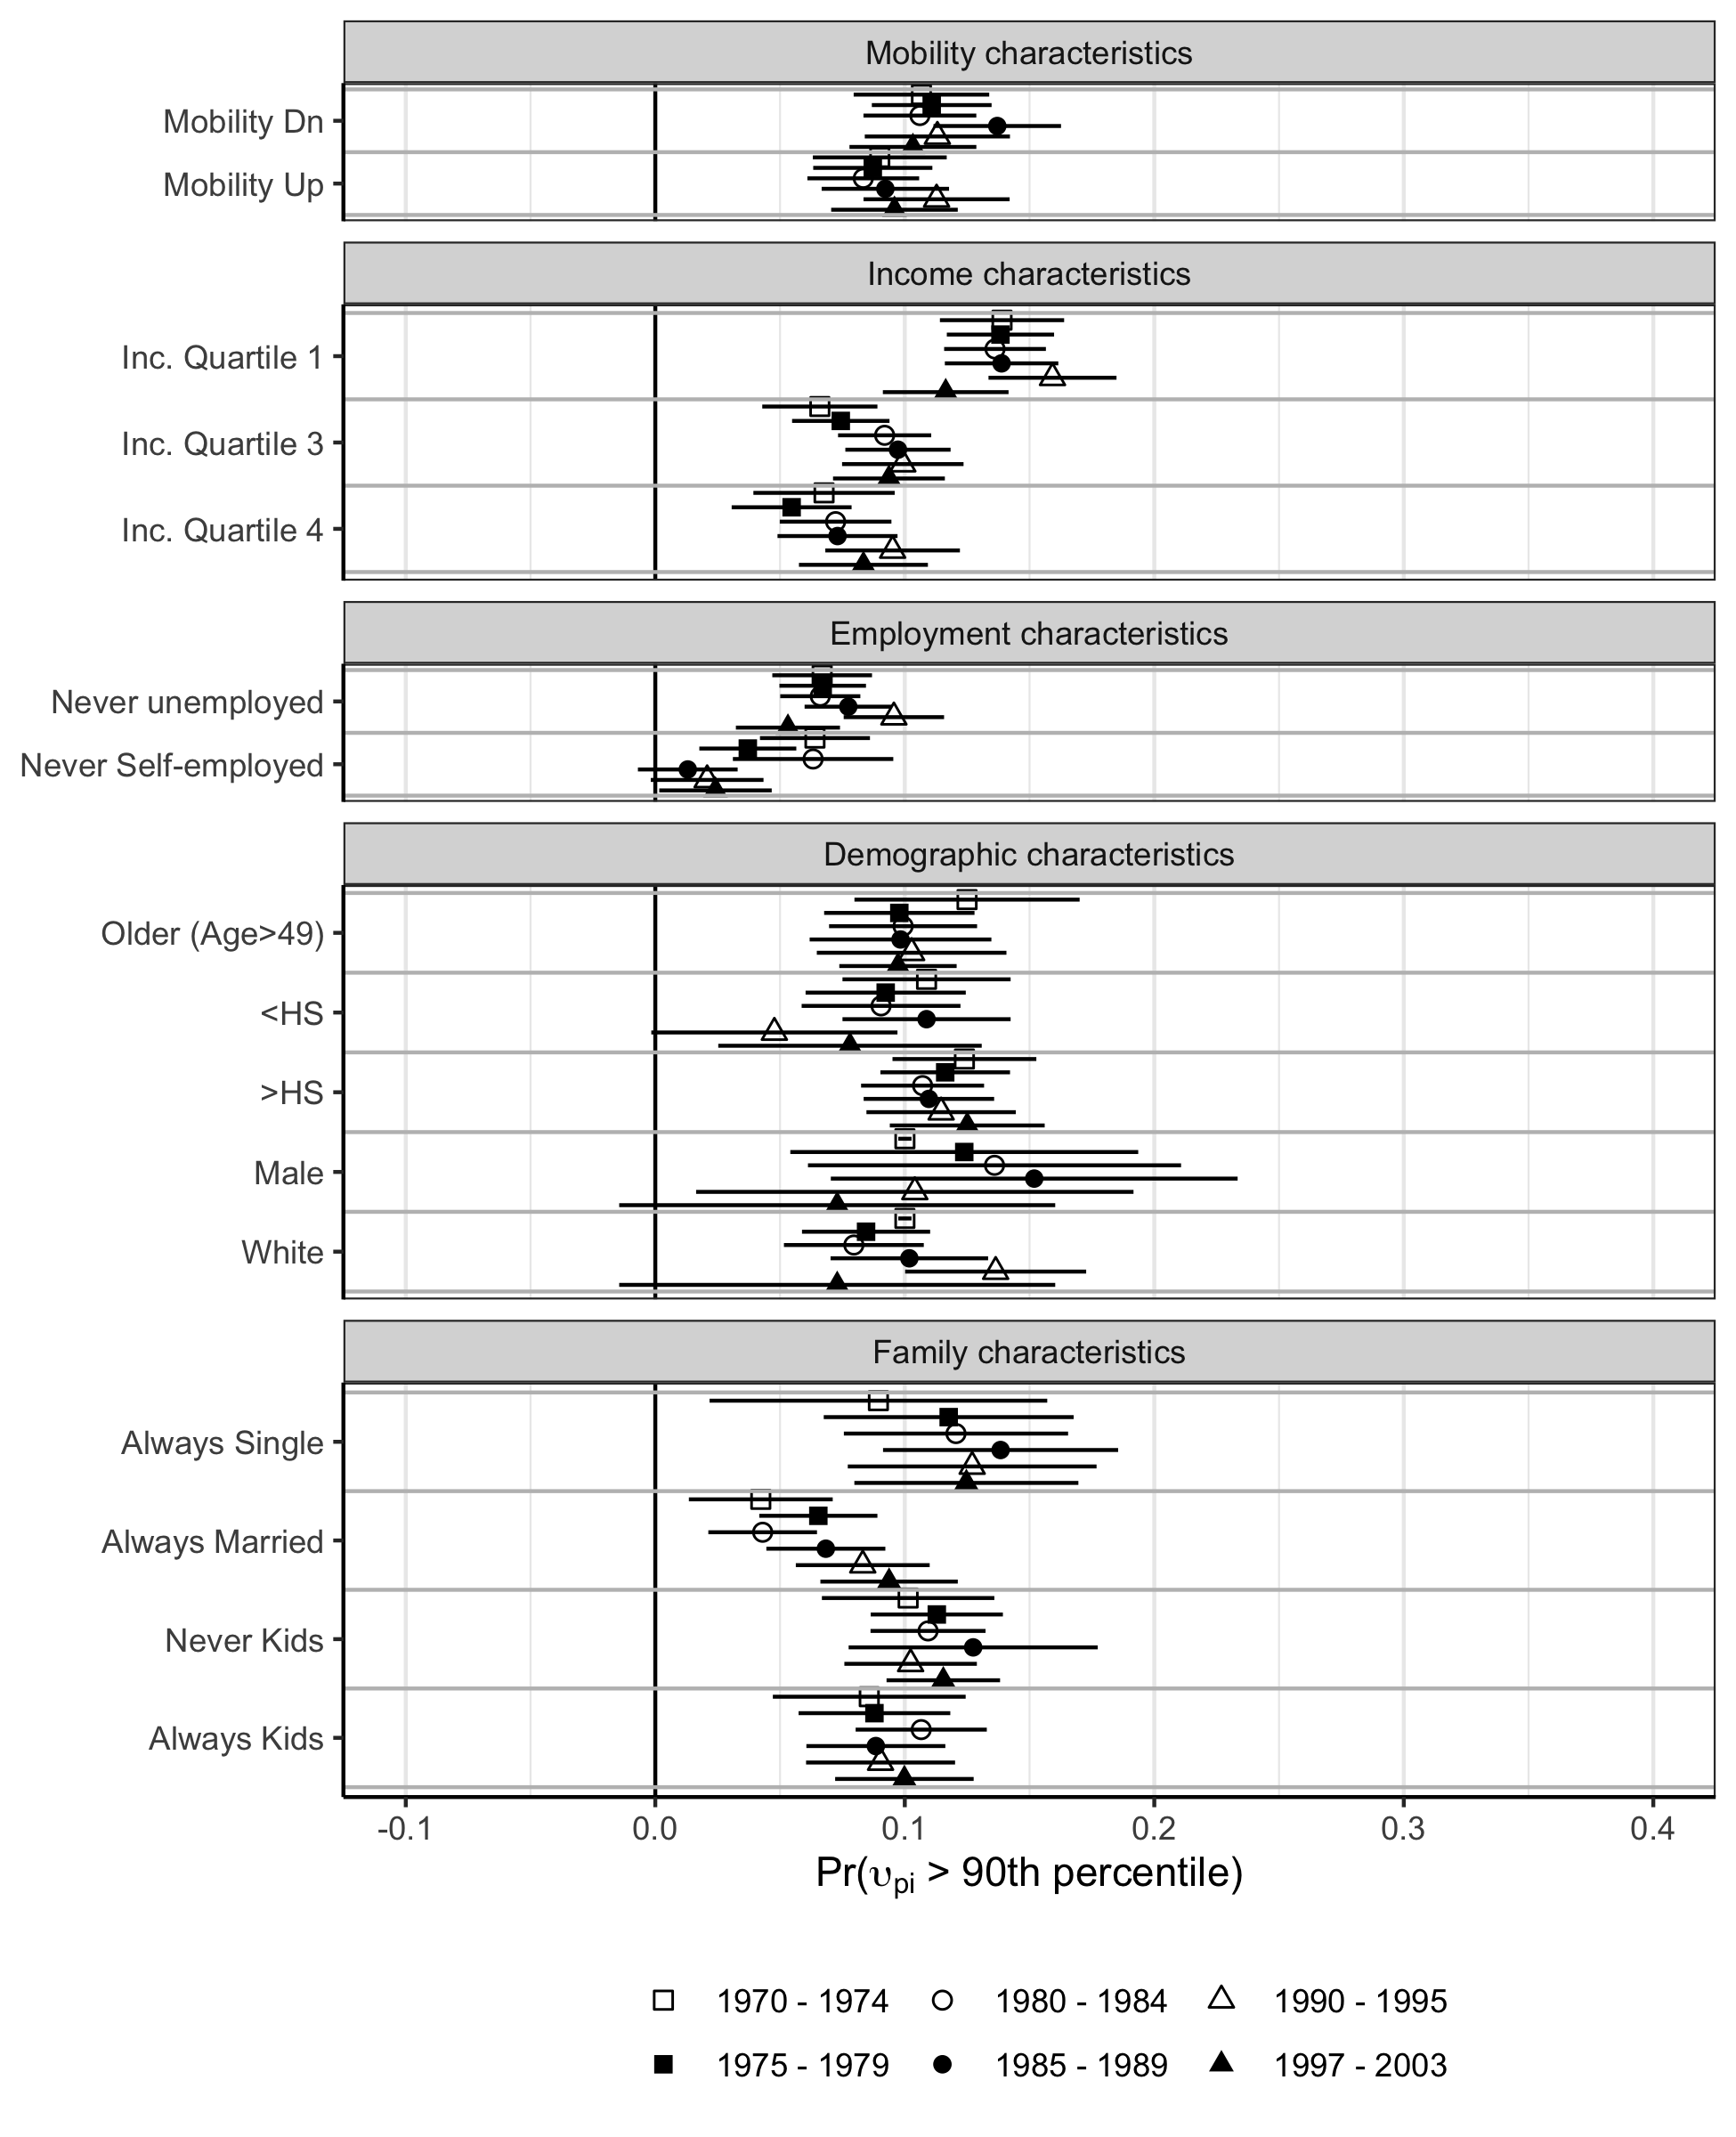
\includegraphics{../graphs/lpm_fe_pr_high_vol_rel_90.png}}
    \label{pr_high_vol}
    \\
    \raggedright{\footnotesize{Note: Graph illustrates the predicted probability of experiencing high income volatility from model \ref{lpm}, as shown in table \ref{lpm_fe_period}.  The interpretation is change over time within each category in the probability of high income volatility relative to the reference category.  For example, the reference category for always single or always married is change in marital status.}}
\end{figure}

\begin{figure}[htp!]
    \centering
    \caption{Index of trends in income volatility and distribution of volatility}
    \resizebox{.9\textwidth}{!}{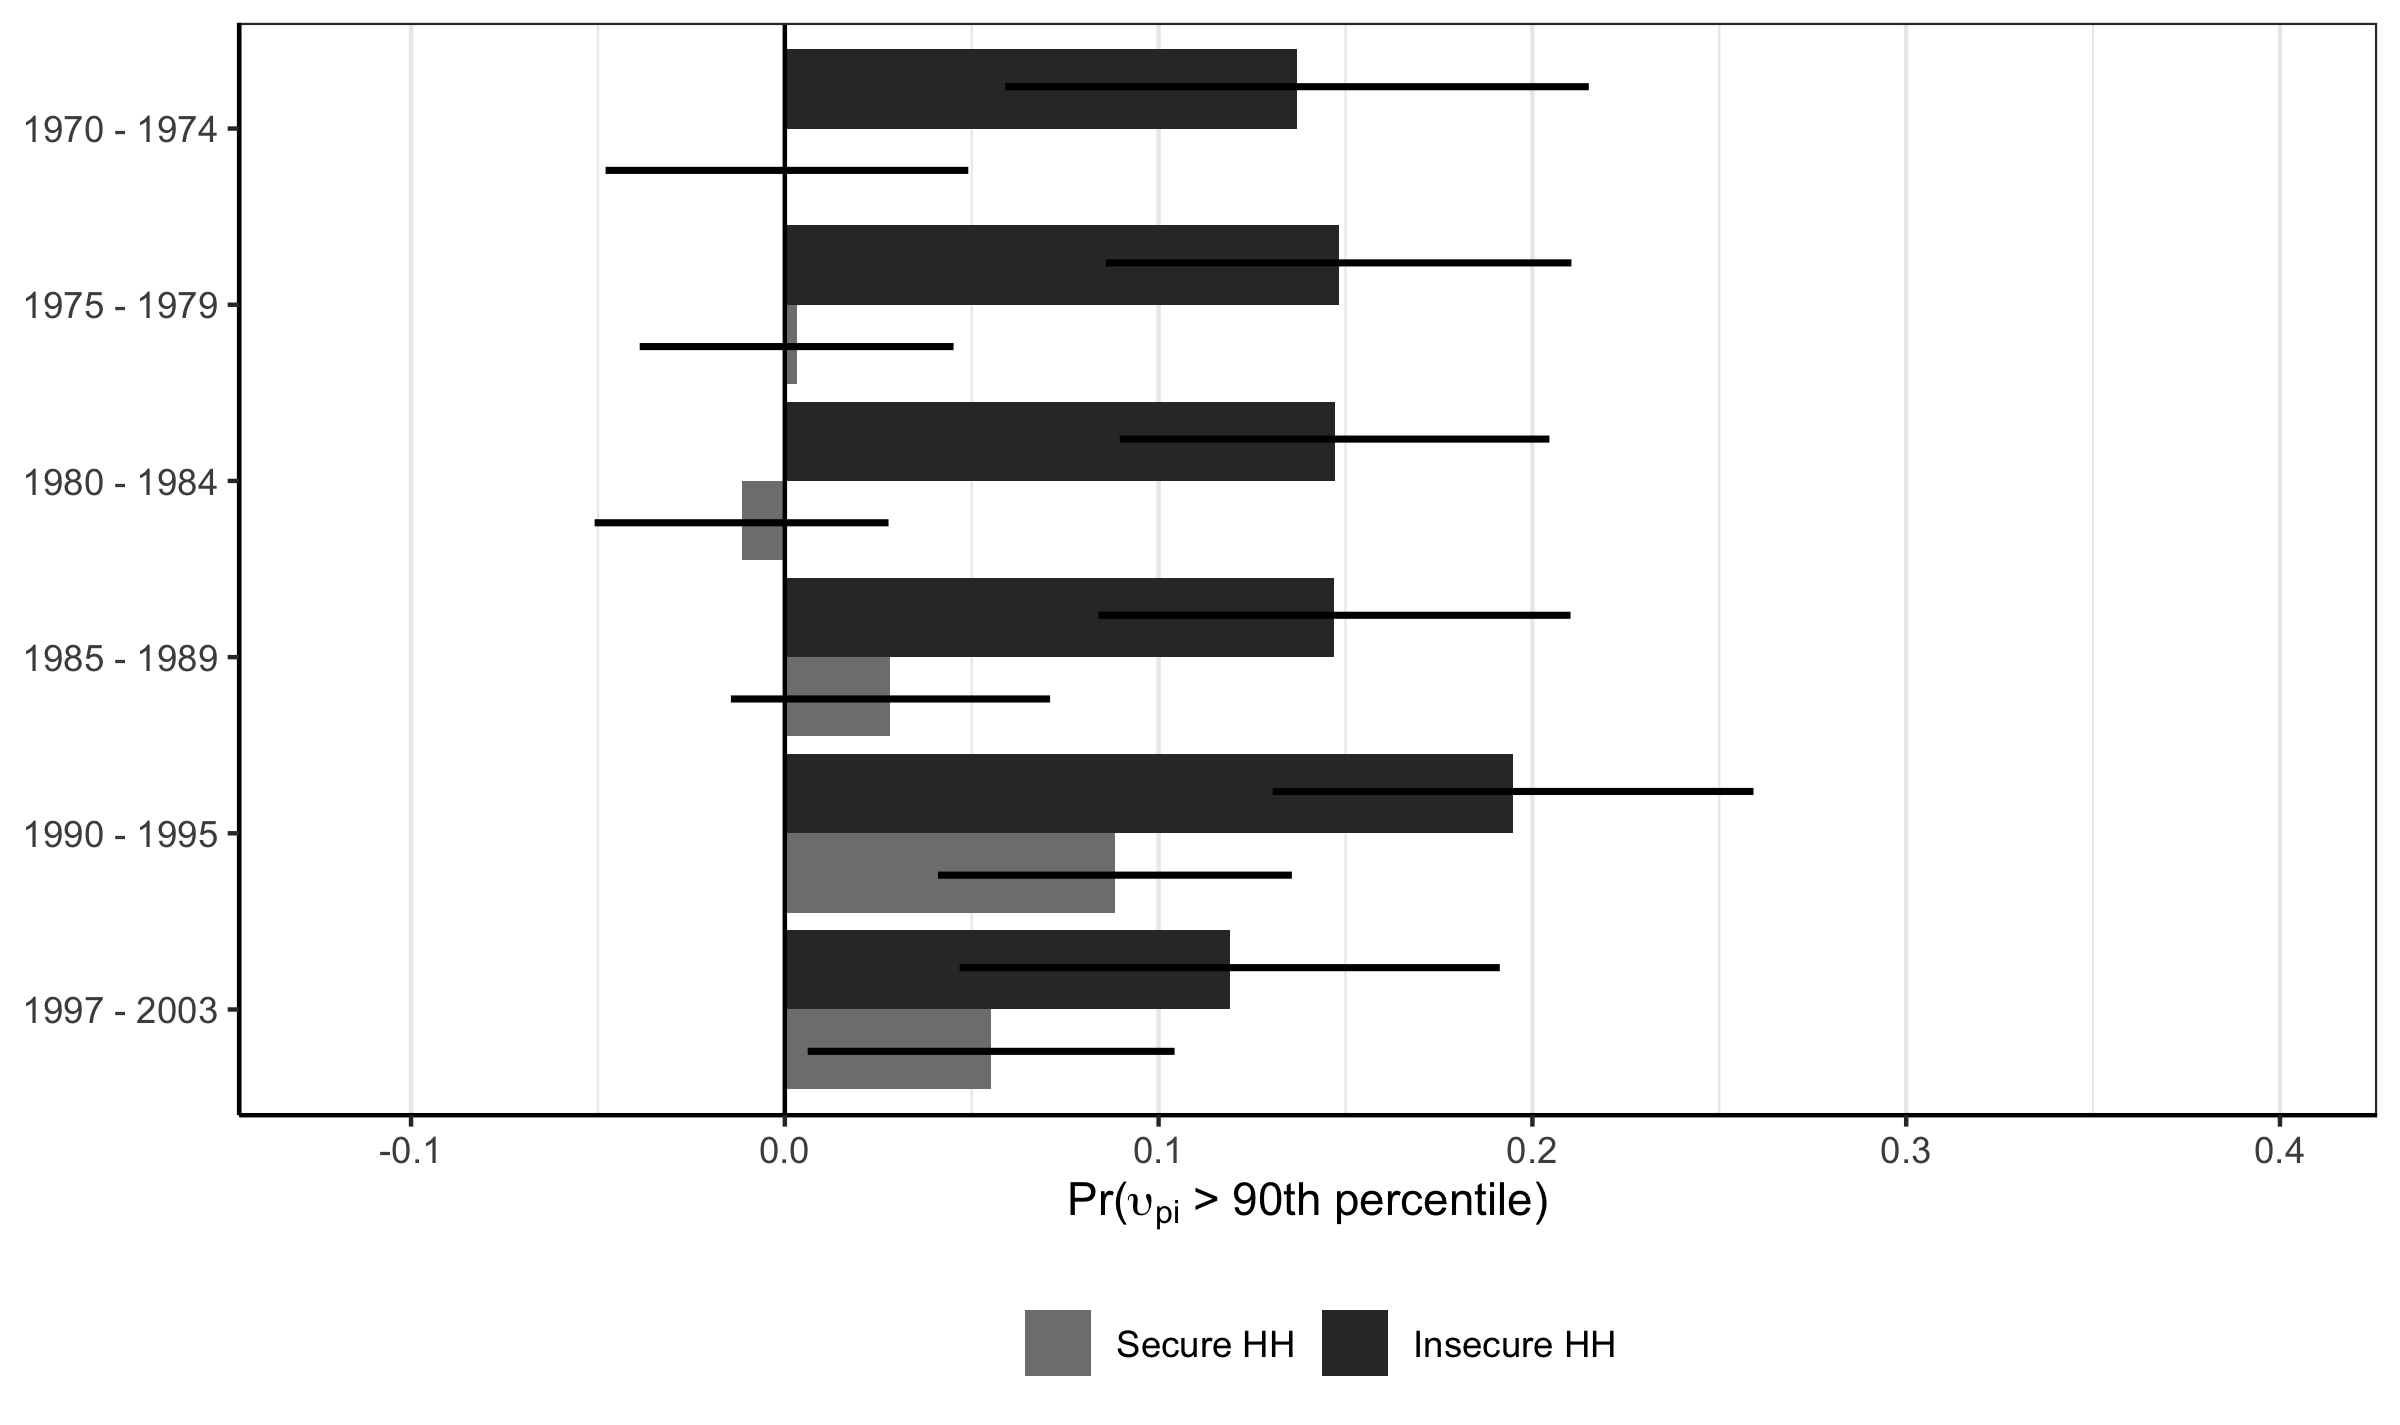
\includegraphics{../graphs/lpm_fe_pr_high_vol_groups_bar_90.png}}
    \label{pr_high_vol_groups}
    \\
    \raggedright{\footnotesize{Note: Graph illustrates the predicted probability of experiencing high income volatility over time by household characteristics from linear probability models with fixed effects, as shown in table \ref{lpm_fe_period}, which is derived from model \ref{lpm_fe_period}.  Controlling for gender, race, age, children in the household, self-employment, and mobility, which are set to their baseline values, ``Secure HH'' is defined as a household that is always married, has a high level of education ($>$ HS), is in the top income quartile, and never unemployed.  ``Insecure HH'' is defined as a household that are always single, has a low level of education ($<$ HS), is in the bottom income quartile, and has experienced unemployment.}}
\end{figure}


\clearpage
%%%%%%%%%%%%%%%%%%%%%%%%%%%%%%%%
% APPENDIX
%%%%%%%%%%%%%%%%%%%%%%%%%%%%%%%%

\appendix
\setcounter{table}{0}
\setcounter{figure}{0}
\renewcommand*\thetable{\Alph{section}.\arabic{table}}
\renewcommand*\thefigure{\Alph{section}.\arabic{figure}}
\section{Appendix}
\label{appendix_a}

\begin{table}
    \caption{Determinants of experiencing high income volatility over time, parameter estimates from a linear probability model with fixed effects, as shown in figure \ref{pr_high_vol}}

\begin{center}
\begin{minipage}[t]{.41\linewidth}
    \vspace{0pt}
    \resizebox{\textwidth}{!}{
\begin{tabular}{@{\extracolsep{5pt}}lD{.}{.}{-3} } 
\\[-1.8ex]\hline 
\hline \\ [-1.8ex] \multicolumn{1}{l}{Variables} & \multicolumn{1}{c}{$\beta$} \\
\hline \\[-1.8ex] 
 \emph{Income mobility:} & \\
                   Downward mobility ($\Delta \hat{y}_{pi} < -5$) & 0.007$ $(0.015) \\ 
  Downward mobility x 1975 $-$ 1979 & 0.004$ $(0.019) \\ 
  Downward mobility x 1980 $-$ 1984 & -0.001$ $(0.019) \\ 
  Downward mobility x 1985 $-$ 1989 & 0.032$ $(0.020) \\ 
  Downward mobility x 1990 $-$ 1996 & 0.007$ $(0.021) \\ 
  Downward mobility x 1997 $-$ 2003 & -0.004$ $(0.020) \\ 
  Upward mobility ($\Delta \hat{y}_{pi} > 5)$ & -0.011$ $(0.014) \\ 
  Upward mobility x 1975 $-$ 1979 & -0.003$ $(0.019) \\ 
  Upward mobility x 1980 $-$ 1984 & -0.007$ $(0.019) \\ 
  Upward mobility x 1985 $-$ 1989 & 0.002$ $(0.020) \\ 
  Upward mobility x 1990 $-$ 1996 & 0.024$ $(0.021) \\ 
  Upward mobility x 1997 $-$ 2003 & 0.006$ $(0.020) \\ 
  & \\ 
                  \emph{Income quartile at start:} & \\
                  Income quartile 1 & 0.041$ $(0.013) \\ 
  Income quartile 1 x 1975 $-$ 1979 & -0.001$ $(0.016) \\ 
  Income quartile 1 x 1980 $-$ 1984 & -0.003$ $(0.017) \\ 
  Income quartile 1 x 1985 $-$ 1989 & -0.000$ $(0.018) \\ 
  Income quartile 1 x 1990 $-$ 1996 & 0.021$ $(0.019) \\ 
  Income quartile 1 x 1997 $-$ 2003 & -0.024$ $(0.019) \\ 
  Income quartile 3 & -0.036$ $(0.012) \\ 
  Income quartile 3 x 1975 $-$ 1979 & 0.009$ $(0.015) \\ 
  Income quartile 3 x 1980 $-$ 1984 & 0.027$ $(0.015) \\ 
  Income quartile 3 x 1985 $-$ 1989 & 0.033$ $(0.016) \\ 
  Income quartile 3 x 1990 $-$ 1996 & 0.035$ $(0.018) \\ 
  Income quartile 3 x 1997 $-$ 2003 & 0.029$ $(0.017) \\ 
  Income quartile 4 & -0.034$ $(0.015) \\ 
  Income quartile 4 x 1975 $-$ 1979 & -0.014$ $(0.017) \\ 
  Income quartile 4 x 1980 $-$ 1984 & 0.005$ $(0.018) \\ 
  Income quartile 4 x 1985 $-$ 1989 & 0.006$ $(0.019) \\ 
  Income quartile 4 x 1990 $-$ 1996 & 0.029$ $(0.020) \\ 
  Income quartile 4 x 1997 $-$ 2003 & 0.017$ $(0.020) \\ 
  & \\ 
               \emph{Demographic characteristics:} & \\
               White &  \\ 
  White x 1975 $-$ 1979 & -0.016$ $(0.014) \\ 
  White x 1980 $-$ 1984 & -0.022$ $(0.015) \\ 
  White x 1985 $-$ 1989 & 0.002$ $(0.017) \\ 
  White x 1990 $-$ 1996 & 0.038$ $(0.019) \\ 
  White x 1997 $-$ 2003 & 0.048$ $(0.020) \\ 
  Male &  \\ 
  Male x 1975 $-$ 1979 & 0.025$ $(0.037) \\ 
  Male x 1980 $-$ 1984 & 0.038$ $(0.040) \\ 
  Male x 1985 $-$ 1989 & 0.055$ $(0.044) \\ 
  Male x 1990 $-$ 1996 & 0.004$ $(0.047) \\ 
  Male x 1997 $-$ 2003 & -0.029$ $(0.047) \\ 
  Older (Age $>$ 49) & 0.026$ $(0.024) \\ 
  Older x 1975 $-$ 1979 & -0.029$ $(0.027) \\ 
  Older x 1980 $-$ 1984 & -0.027$ $(0.029) \\ 
  Older x 1985 $-$ 1989 & -0.028$ $(0.031) \\ 
  Older x 1990 $-$ 1996 & -0.023$ $(0.032) \\ 
  Older x 1997 $-$ 2003 & -0.029$ $(0.027) \\ 
 \hline \\[-1.8ex] 
\hline 
\hline \\[-1.8ex] 
\textit{Note:}  & \multicolumn{1}{l}{\emph{continued...}} \\ 
\end{tabular} 
}
\end{minipage}%
\begin{minipage}[t]{.48\linewidth}
    \vspace{0pt}
    \resizebox{\textwidth}{!}{
\begin{tabular}{@{\extracolsep{5pt}}lD{.}{.}{-3} } 
\\[-1.8ex]\hline 
\hline \\ [-1.8ex] \multicolumn{1}{l}{Variables \emph{(continued)}} & \multicolumn{1}{c}{$\beta$} \\
\hline \\[-1.8ex] 
 \emph{Education:} & \\
                  Less than HS & 0.009$ $(0.018) \\ 
  Less than HS x 1975 $-$ 1979 & -0.017$ $(0.015) \\ 
  Less than HS x 1980 $-$ 1984 & -0.019$ $(0.017) \\ 
  Less than HS x 1985 $-$ 1989 & -0.041$ $(0.021) \\ 
  Less than HS x 1990 $-$ 1996 & -0.064$ $(0.027) \\ 
  Less than HS x 1997 $-$ 2003 & -0.032$ $(0.029) \\ 
  More than HS & 0.025$ $(0.015) \\ 
  More than HS x 1975 $-$ 1979 & -0.008$ $(0.014) \\ 
  More than HS x 1980 $-$ 1984 & -0.018$ $(0.015) \\ 
  More than HS x 1985 $-$ 1989 & -0.015$ $(0.016) \\ 
  More than HS x 1990 $-$ 1996 & -0.010$ $(0.018) \\ 
  More than HS x 1997 $-$ 2003 & 0.001$ $(0.018) \\ 
  & \\ 
                 \emph{Employment characteristics:} & \\
                 Never unemployed & -0.035$ $(0.011) \\ 
  Never unemployed x 1975 $-$ 1979 & 0.000$ $(0.012) \\ 
  Never unemployed x 1980 $-$ 1984 & -0.001$ $(0.012) \\ 
  Never unemployed x 1985 $-$ 1989 & 0.011$ $(0.014) \\ 
  Never unemployed x 1990 $-$ 1996 & 0.030$ $(0.015) \\ 
  Never unemployed x 1997 $-$ 2003 & -0.014$ $(0.015) \\ 
  Never self-unemployed & -0.038$ $(0.012) \\ 
  Never self-unemployed x 1975 $-$ 1979 & -0.028$ $(0.012) \\ 
  Never self-unemployed x 1980 $-$ 1984 & -0.034$ $(0.013) \\ 
  Never self-unemployed x 1985 $-$ 1989 & -0.054$ $(0.014) \\ 
  Never self-unemployed x 1990 $-$ 1996 & -0.045$ $(0.016) \\ 
  Never self-unemployed x 1997 $-$ 2003 & -0.042$ $(0.016) \\ 
  & \\ 
                  \emph{Family characteristics:} & \\
                  Always single & -0.011$ $(0.036) \\ 
  Always single x 1975 $-$ 1979 & 0.030$ $(0.037) \\ 
  Always single x 1980 $-$ 1984 & 0.033$ $(0.039) \\ 
  Always single x 1985 $-$ 1989 & 0.052$ $(0.042) \\ 
  Always single x 1990 $-$ 1996 & 0.040$ $(0.044) \\ 
  Always single x 1997 $-$ 2003 & 0.037$ $(0.043) \\ 
  Always married & -0.061$ $(0.015) \\ 
  Always married x 1975 $-$ 1979 & 0.024$ $(0.016) \\ 
  Always married x 1980 $-$ 1984 & 0.001$ $(0.017) \\ 
  Always married x 1985 $-$ 1989 & 0.027$ $(0.019) \\ 
  Always married x 1990 $-$ 1996 & 0.043$ $(0.020) \\ 
  Always married x 1997 $-$ 2003 & 0.054$ $(0.021) \\ 
  Never kids & 0.001$ $(0.019) \\ 
  Never kids x 1975 $-$ 1979 & 0.012$ $(0.020) \\ 
  Never kids x 1980 $-$ 1984 & 0.008$ $(0.021) \\ 
  Never kids x 1985 $-$ 1989 & -0.021$ $(0.022) \\ 
  Never kids x 1990 $-$ 1996 & 0.001$ $(0.023) \\ 
  Never kids x 1997 $-$ 2003 & 0.015$ $(0.022) \\ 
  Always kids & -0.015$ $(0.021) \\ 
  Always kids x 1975 $-$ 1979 & 0.002$ $(0.021) \\ 
  Always kids x 1980 $-$ 1984 & 0.022$ $(0.023) \\ 
  Always kids x 1985 $-$ 1989 & 0.003$ $(0.024) \\ 
  Always kids x 1990 $-$ 1996 & 0.005$ $(0.026) \\ 
  Always kids x 1997 $-$ 2003 & 0.015$ $(0.025) \\ 
  & \\ 
                         \emph{Study period beginning:} & \\
                         1975 $-$ 1979 & -0.001$ $(0.054) \\ 
  1980 $-$ 1984 & 0.005$ $(0.056) \\ 
  1985 $-$ 1989 & -0.028$ $(0.060) \\ 
  1990 $-$ 1996 & -0.056$ $(0.065) \\ 
  1997 $-$ 2003 & -0.004$ $(0.064) \\ 
  & \\ 
                    Constant & 0.100$ $(0.001) \\ 
 \hline \\[-1.8ex] 
Observations & \multicolumn{1}{c}{48,718} \\ 
R$^{2}$ & \multicolumn{1}{c}{0.009} \\ 
\hline 
\hline \\[-1.8ex] 
\textit{Note:}  & \multicolumn{1}{l}{Standard errors in parenthesis.} \\ 
\end{tabular} 
}
\end{minipage}%
\end{center}

\label{lpm_fe_period}
\end{table}


\end{document}
